\chapter{Реализация и экспериментальная проверка системы ролевой игры с виртуальным мастером}

В данной главе описывается реализация разработанной системы, выбор инструментальных средств, структура программного обеспечения, основные сценарии работы пользователя и результаты тестирования.





Для реализации системы ролевой игры с виртуальным мастером выбраны следующие инструментальные средства:

\begin{itemize}
	\item \textbf{Язык программирования Python 3.11} --- выбран как основной язык разработки благодаря богатой экосистеме библиотек для работы с большими языковыми моделями, поддержке асинхронного программирования и простоте разработки.
	
	\item \textbf{Библиотека aiohttp} --- используется для асинхронных HTTP-запросов к API больших языковых моделей, что обеспечивает возможность параллельной обработки запросов и повышает производительность системы.
	
	\item \textbf{Библиотека numpy} --- используется для работы с векторными представлениями эмоций и намерений персонажей, обеспечивая эффективные вычисления над массивами.
	
	\item \textbf{Библиотека python-dotenv} --- используется для загрузки конфигурации из переменных окружения, обеспечивая безопасное хранение API-ключей.
	
	\item \textbf{Библиотека pyyaml} --- используется для чтения конфигурационных файлов в формате YAML, позволяя гибко настраивать параметры взаимодействия с большими языковыми моделями.
\end{itemize}

Выбор данных инструментальных средств обусловлен требованиями к системе: необходимостью асинхронной обработки запросов к API, работы с векторными представлениями данных и гибкой конфигурации системы.




\section{Состав и структура реализованного программного обеспечения}

Реализованная система представляет собой консольное приложение для Windows, Linux и macOS, написанное на языке Python. Система состоит из следующих основных компонентов:

\subsection{Структура проекта}

Проект организован в виде модульной структуры:

\begin{itemize}
	\item \texttt{src/main.py} --- точка входа в приложение, содержащая функцию \texttt{main()} для инициализации и запуска игры.
	
	\item \texttt{src/game/} --- основной пакет, содержащий логику игры:
	\begin{itemize}
		\item \texttt{game.py} --- классы \texttt{Game} и \texttt{Plot} для управления игровым циклом.
		\item \texttt{scene.py} --- класс \texttt{Scene} и связанные классы для управления сценами.
		\item \texttt{characters.py} --- классы \texttt{Character}, \texttt{MCharacter}, \texttt{PCharacter} и \texttt{Stats} для представления персонажей.
		\item \texttt{director.py} --- класс \texttt{Director} для выдачи директив.
		\item \texttt{storyteller.py} --- класс \texttt{Storyteller} для генерации повествования.
		\item \texttt{dice.py} --- класс \texttt{Dice} для разрешения действий.
		\item \texttt{story.py} --- определения сюжетов и сцен.
		\item \texttt{base\_agent.py} --- базовый класс агента и функция создания агентов.
	\end{itemize}
	
	\item \texttt{src/game/core/} --- пакет с базовыми компонентами:
	\begin{itemize}
		\item \texttt{agent.py} --- абстрактный класс \texttt{Agent}.
		\item \texttt{brain.py} --- классы \texttt{Brain} и \texttt{MoralScheme} для управления эмоциями.
		\item \texttt{interface.py} --- класс \texttt{Interface} для взаимодействия с API больших языковых моделей.
		\item \texttt{role.py} --- классы \texttt{Role} и \texttt{Section} для определения ролей персонажей.
		\item \texttt{prompts.py} --- предопределённые роли персонажей.
		\item \texttt{constants.py} --- константы системы (пространства эмоций и намерений).
		\item \texttt{config.py} --- функции для загрузки конфигурации.
		\item \texttt{utils.py} --- вспомогательные функции.
		\item \texttt{manager.py} --- класс \texttt{AgentManager} для управления агентами.
	\end{itemize}
\end{itemize}

\subsection{Конфигурационные файлы}

\begin{itemize}
	\item \texttt{config.yaml} --- файл конфигурации, содержащий настройки для взаимодействия с большими языковыми моделями (провайдер, API ключ, базовый URL, модель).
	
	\item \texttt{.env} --- файл с переменными окружения для хранения API-ключей (не включается в систему контроля версий).
	
	\item \texttt{crequirements.txt} --- файл зависимостей проекта для установки через pip.
\end{itemize}




\section{Основные сценарии работы пользователя}

Система предназначена для использования игроком, который взаимодействует с виртуальным мастером и неигровыми персонажами через консольный интерфейс.

\subsection*{Запуск игры и начало сцены}

\begin{enumerate}
	\item Пользователь запускает приложение, выполняя команду \texttt{python src/main.py}.
	
	\item Система инициализирует компоненты: загружает конфигурацию из \texttt{config.yaml}, создаёт интерфейс для взаимодействия с большими языковыми моделями, инициализирует персонажей и сцены.
	
	\item \texttt{Storyteller} генерирует начальное описание первой сцены и выводит его в консоль в обрамлённом виде.
	
	\item Система отображает список присутствующих неигровых персонажей в сцене.
\end{enumerate}

\subsection*{Взаимодействие с неигровыми персонажами}

\begin{enumerate}
	\item \texttt{Director} анализирует текущее состояние игры и выдаёт директиву одному из персонажей (игроку или неигровому персонажу).
	
	\item Если директива выдана игроку:
	\begin{enumerate}
		\item Система выводит директиву в консоль и запрашивает действие игрока.
		\item Игрок вводит действие через консоль.
		\item \texttt{PCharacter.judge()} проверяет соответствие действия предыстории персонажа.
		\item Если действие не соответствует, система выводит замечание и запрашивает новое действие.
	\end{enumerate}
	
	\item Если директива выдана неигровому персонажу:
	\begin{enumerate}
		\item \texttt{MCharacter.get\_replic\_to()} вызывает \texttt{Agent.generate\_reply()} для генерации ответа.
		\item Агент анализирует намерения и эмоции в директиве, обновляет моральную схему и генерирует ответ.
	\end{enumerate}
	
	\item \texttt{SceneJudge} проверяет корректность действия на соответствие сюжету.
	
	\item При необходимости \texttt{Dice} определяет и выполняет механическую проверку действия (бросок кубика).
	
	\item \texttt{SceneJudge} определяет, какие персонажи восприняли действие.
	
	\item Память всех воспринявших действие персонажей обновляется.
	
	\item \texttt{Storyteller} генерирует повествование действия и выводит его в консоль.
\end{enumerate}

\subsection*{Завершение сцены и переход к следующей}

\begin{enumerate}
	\item После каждого действия \texttt{SceneChanger} проверяет, завершена ли текущая сцена.
	
	\item Если сцена завершена, система переходит к следующей сцене в сюжете.
	
	\item \texttt{Storyteller} генерирует начальное описание новой сцены.
	
	\item Игровой цикл продолжается с новой сцены.
\end{enumerate}





\section{Тестирование системы}

Главная задача тестирования --- проверка работоспособности системы в условиях, приближенных к реальным.
Для этого, с учетом основных требований к системе, были составлены типовые запросы, соответствующие главным пользовательским сценариями.
Основными требованиями системы являются:
\begin{itemize}
	\item валидация действий игрока
	\item оценка сложности действий и проверка успеха его выполнения
	\item сопровождение игрока по сюжету
	\item реализация вариативного и адаптивного взаимодействия с неигровыми персонажами
	\item неигровые персонажи проявляют инициативу действий
\end{itemize}

Далее приведены реализованные тестовые сценарии.

\subsection*{Стандратное действие игрока}
\begin{itemize}
	\item \textbf{Ввод игрока:} "Take a look of a tavern"
	\item \textbf{Ожидаемая реакция: } Игра дает описание таверны.
	\item \textbf{Полученный ответ: } \ref{pic:test1-1}. Неигровые персонажи настороженно реагируют на любопытный взгля игрока.

\end{itemize}
\begin{figure}[h!]
	\centering
	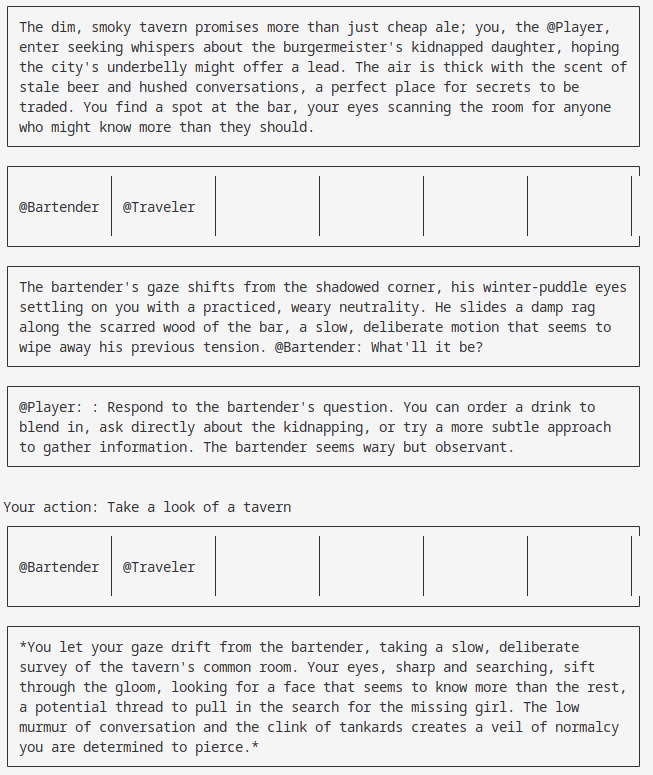
\includegraphics[width=0.8\linewidth]{img/test1.1.png}
	\caption{Неинтерактивное действие}
	\label{pic:test1-1}
\end{figure}

\subsection*{Стандратное действие игрока (взаимодействие с миром)}
\begin{itemize}
	\item \textbf{Ввод игрока:} "Buy a tankard of ale"
	\item \textbf{Ожидаемая реакция: } Бармен подает игроку напиток.
	\item \textbf{Полученный ответ: } \ref{pic:test1-2}. Игрок просит напиток. Бармен выполняет дейтсвие, и подает игроку напиток. Второй неигровой персонаж проявляет инициативу и взаимодействует с игроков.

\end{itemize}
\begin{figure}[h!]
	\centering
	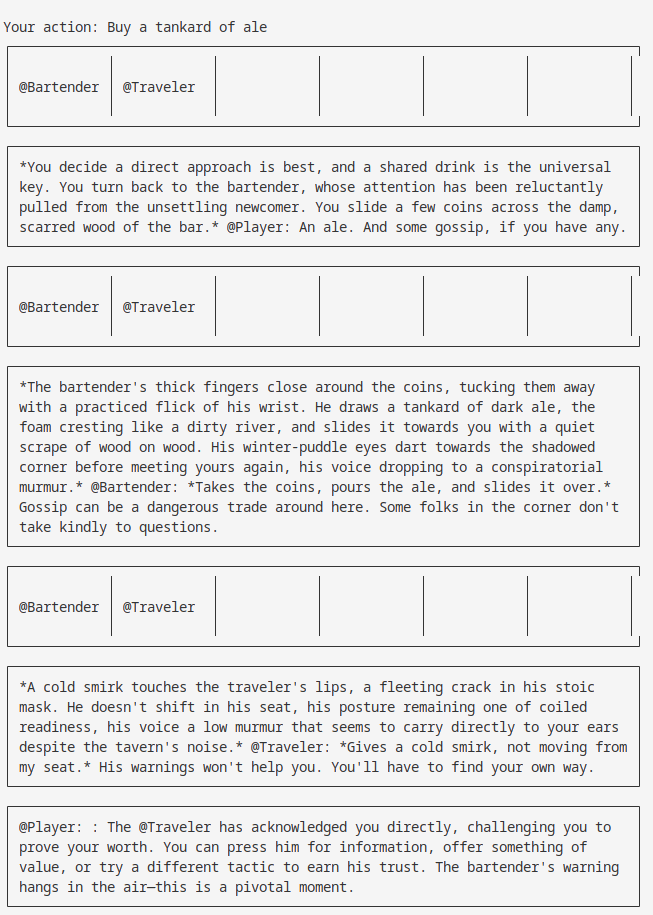
\includegraphics[width=0.8\linewidth]{img/test1.2.png}
	\caption{Покупка напитка у Бармена}
	\label{pic:test1-2}
\end{figure}

\subsection*{Неадекватное осуществимое действие игрока}
\begin{itemize}
	\item \textbf{Ввод игрока:} "Jump on the bar counter and do a backflip"
	\item \textbf{Ожидаемая реакция: } Персонаж игрока предпринимает попытку прыжка. Результат не определен.
	\item \textbf{Полученный ответ: } \ref{pic:test1-3}. Мастер игры принимает действие игрока и проводит (вероятностную) проверку на сложность. Игрок не приходоит проверку, и его действие проваливается, он неловко падает.

\end{itemize}
\begin{figure}[h!]
	\centering
	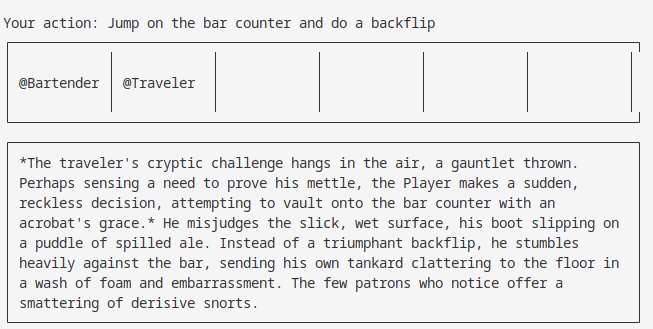
\includegraphics[width=0.8\linewidth]{img/test1.3.png}
	\caption{Сальто с барной стойки}
	\label{pic:test1-3}
\end{figure}

\subsection*{Неосуществимое действие игрока}
\begin{itemize}
	\item \textbf{Ввод игрока:} "Drop an atmomic bomb"
	\item \textbf{Ожидаемая реакция: } Игра отвергает невыполнимый запрос игрока.
	\item \textbf{Полученный ответ: } \ref{pic:test1-4}. Действие игрока не проходит валидацию и отвергается. Игра дает пояснение, что описанное действие невозмонжо в текущем игровом сеттинге и окружении.

\end{itemize}
\begin{figure}[h!]
	\centering
	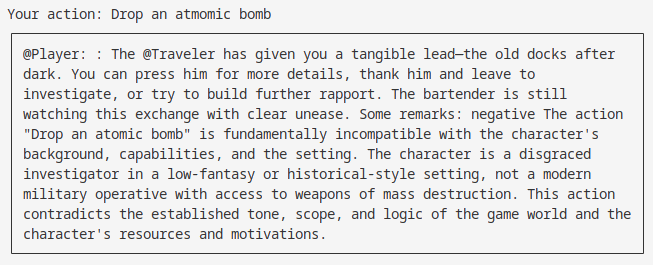
\includegraphics[width=0.8\linewidth]{img/test1.4.png}
	\caption{Сбросить атомную бомбу}
	\label{pic:test1-4}
\end{figure}

\section{Сравнение реализованного программного обеспечения с существующими аналогами}

\subsection{Преимущества разработанной системы}

\begin{enumerate}
	\item \textbf{Структурированное управление состоянием игры}: в отличие от чисто генеративных решений, система поддерживает явное представление состояния игры, что обеспечивает согласованность происходящего.
	
	\item \textbf{Контроль действий игрока}: система проверяет соответствие действий предыстории персонажа, логике мира и правилам игры, что предотвращает разрушение игрового процесса.
	
	\item \textbf{Интеграция механических правил}: система интегрирует броски кубиков и проверки характеристик с генерацией повествования, обеспечивая согласованность между механическими правилами и описанием происходящего.
	
	\item \textbf{Эмоциональное моделирование персонажей}: система управляет эмоциональным состоянием неигровых персонажей, обеспечивая более реалистичное и непредсказуемое их поведение.
	
	\item \textbf{Механизм выдачи директив}: система использует компонент директора для координации действий неигровых персонажей, обеспечивая баланс между свободой действий игрока и следованием задуманному сюжету.
\end{enumerate}

\subsection{Ограничения разработанной системы}

\begin{enumerate}
	\item \textbf{Зависимость от API больших языковых моделей}: система требует постоянного доступа к интернету и API ключа, что может ограничивать доступность.
	
	\item \textbf{Задержки при генерации}: использование больших языковых моделей для генерации ответов может приводить к задержкам в игровом процессе.
	
	\item \textbf{Ограниченность консольного интерфейса}: в отличие от веб-приложений, консольный интерфейс менее удобен для визуализации игрового процесса.
\end{enumerate}



\section{Выводы}

В результате реализации и экспериментальной проверки системы ролевой игры с виртуальным мастером получены следующие практические результаты:

\begin{enumerate}
	\item Реализована полнофункциональная система ролевой игры с виртуальным мастером на языке Python, включающая все разработанные компоненты: управление игровым циклом, генерацию повествования, управление персонажами, эмоциональное моделирование, разрешение действий и контроль корректности действий.
  
  \item Было проведено тестирование системы, основываясь на обработке краевых случаев.
	
	\item Проведено сравнение разработанной системы с существующими коммерческими аналогами. Система превосходит аналоги по следующим характеристикам: контроль действий игрока, структурированное представление состояния мира, интеграция механических правил, управление персонажами с учётом эмоционального состояния, проверка корректности действий.
	
	\item Система демонстрирует более структурированный и контролируемый игровой процесс по сравнению с существующими генеративными решениями, сохраняя при этом гибкость и вариативность повествования, характерные для традиционных ролевых игр с живым мастером.
\end{enumerate}

Разработанная система представляет собой практическую реализацию подхода к созданию виртуальных мастеров для ролевых игр, объединяющего структурированное управление состоянием игры с генеративными возможностями больших языковых моделей.

%%% Local Variables:
%%% TeX-engine: xetex
%%% eval: (setq-local TeX-master (concat "../" (seq-find (-cut string-match ".*-3-pz\.tex$" <>) (directory-files ".."))))
%%% End:
